% Provenance (never printed): see sources/outline_sources.md (Year 2: ore deposits ---
% magmatic, hydrothermal, sedimentary and supergene deposits; grade and tonnage; exploration).
% Deposit descriptions from the USGS Mineral Deposit Models for Resource Assessment
% (Scientific Investigations Report 2010-5070, chapters A, B, C, E, I, L, N, O, Q), USGS
% Open-File Report 03-077 (orogenic gold) and Grabreck et al. 2022 (kimberlites); the grade and
% tonnage data of the world's porphyry copper deposits from USGS Open-File Report 2008-1155
% (dataset bachelor-2-porphyry-cu). Ledger rows in sources/ledger/book4.md; curves and numbers
% from figdata/bachelor-2/ores.py and the Book 4 second-writer scratch calculator calc/ch29.py.
% Geology and sourced numbers only: no advocacy.
\chapter{矿床}\label{ch:b2:ore-deposits}

铜约占地壳的 \qty{0.006}{\percent}，而开采的岩石中铜
含量约为 \qty{0.5}{\percent}。因此每座铜矿所在的岩石，铜含量比周围地壳高约八十倍；
每个\omterm{def:b2:ore-deposits:deposit}{矿床}都是某种天然富集作用的结果：\omterm{def:b2:magma-emplacement:magma}{岩浆}分离出硫化物熔体，
热卤水溶解金属并将其沉积于裂隙中，河流把重矿粒与轻矿粒分选开，
雨水淋滤矿体顶部，使铜在下方重新沉淀。本章沿着这些富集作用追踪，
然后测量它们的产物——矿石有多少、品位如何——
并以\omterm{def:b2:ore-deposits:deposit}{矿床}的找寻方式作结。
% ledger: perkins:ore-grades

\begin{recall}
\textbf{来自中学各册}：\omterm{def:b2:ore-deposits:deposit}{矿床}与\omterm{def:b2:ore-deposits:cf}{富集系数}、脉、\omterm{def:b2:ore-deposits:placer}{砂矿}、储量与
资源；洋脊处的热液循环与黑烟囱。\textbf{来自化学各册}：
矿石；溶解度、络离子与氧化还原。\textbf{来自本科一年级分册}：颗粒的沉降
速度与斯托克斯定律；红土；蒸发岩。\textbf{来自
\cref{ch:b2:elements-in-the-earth}}：\omterm{def:b2:elements-in-the-earth:goldschmidt}{亲铜元素}、\omterm{def:b2:elements-in-the-earth:partition}{矿物–熔体
分配系数}。\textbf{来自\cref{ch:b2:magmatic-differentiation}}：\omterm{def:b2:magmatic-differentiation:cumulate}{层状侵入体}与
\omterm{def:b2:magmatic-differentiation:cumulate}{堆晶岩}。\textbf{来自\cref{ch:b2:precambrian-earth}}：\omterm{def:b2:precambrian-earth:bif}{条带状铁建造}、\omterm{def:b2:precambrian-earth:craton}{克拉通}。
\textbf{来自数学各册}：正态分布与对数正态分布，以及正态
分布函数 $\Phi$。
\end{recall}

\section{矿石、品位与富集}\label{sec:b2:ore-deposits:grade}

\begin{definition}[脉石]\label{def:b2:ore-deposits:ore}
矿石中，\emph{脉石}\index{脉石}指一切没有经济价值的部分：
与矿石矿物伴生的造岩矿物、热液矿物与风化矿物，
在选矿时与矿石矿物分离并弃去。
\end{definition}

多数矿石其实是\omterm{def:b2:ore-deposits:ore}{脉石}。在\omterm{def:b2:ore-deposits:hydrothermal}{斑岩铜矿床}（世界主要的铜来源）中，超过
\qty{98}{\percent} 的矿石为\omterm{def:b2:ore-deposits:ore}{脉石}，其余才是铜矿物。
% ledger: usgs10b:share

\begin{definition}[矿石品位、边界品位、矿石量]\label{def:b2:ore-deposits:grade}
一定体积岩石的\emph{矿石品位}\index{矿石品位}是其中有用
元素或矿物的质量分数：贱金属以百分数计，金、银与
铂族元素以克/吨计。\emph{边界品位}\index{边界品位}是岩块被计为矿石的
最低品位；低于它的岩块即为废石。\emph{矿石量}\index{矿石量}指
\omterm{def:b2:ore-deposits:deposit}{矿床}中高于边界品位的岩石质量，
结合其平均品位 $\bar g$，即得所含金属量 $M = T\bar g$。
\end{definition}

因此，\omterm{def:b2:ore-deposits:deposit}{矿床}的\omterm{def:b2:ore-deposits:grade}{矿石量}与品位并非岩石的两个事实，而是
同一问题在给定\omterm{def:b2:ore-deposits:grade}{边界品位}下的两种回答。Batu Hijau 为一座斑岩铜金\omterm{def:b2:ore-deposits:deposit}{矿床}，位于
印度尼西亚，报告数据为\omterm{def:b2:ore-deposits:grade}{矿石量} \qty{914}{Mt}、铜品位 \qty{0.53}{\percent}，高于
\qty{0.3}{\percent} 的\omterm{def:b2:ore-deposits:grade}{边界品位}；在一份世界汇编中，\omterm{def:b2:ore-deposits:grade}{矿石量}为 \qty{1640}{Mt}、品位为 \qty{0.44}{\percent}，
该汇编采用可得的最低\omterm{def:b2:ore-deposits:grade}{边界品位}：降低\omterm{def:b2:ore-deposits:grade}{边界品位}几乎使\omterm{def:b2:ore-deposits:grade}{矿石量}翻倍，
并使平均品位降低。加拿大的 Tom \omterm{def:b2:ore-deposits:deposit}{矿床}是一座沉积型锌铅\omterm{def:b2:ore-deposits:deposit}{矿床}，若将
\omterm{def:b2:ore-deposits:grade}{边界品位}（锌加铅）约降低一个百分点，则储量将增至五倍。
% ledger: usgs10b:cutoffs, usgs08:tonnage-def, usgs10n:sedex

\begin{definition}[富集系数]\label{def:b2:ore-deposits:cf}
矿石中某元素的\emph{富集系数}\index{富集系数}是其品位与参考储库中丰度之比，
即 $\mathrm{CF} = g/a$，其中 $g$ 为品位，$a$ 为丰度，并须注明参考储库：
整个大陆地壳、上部大陆地壳，或成矿母岩。
\end{definition}

\omterm{def:b2:ore-deposits:cf}{富集系数}取决于所选参考。以地壳中 \qty{0.006}{\percent} 的铜为参考，
矿石取 \qty{0.5}{\percent}，得\omterm{def:b2:ore-deposits:cf}{富集系数} 83；若以上部大陆地壳为参考，
丰度为 \qty{28}{ppm}，2008 年斑岩铜矿的平均品位为 \qty{0.44}{\percent}，得 157。金
在上部地壳中丰度为 \qty{1.5}{ng/g}，开采品位仅为每吨几克，其\omterm{def:b2:ore-deposits:cf}{富集系数}达数千；
铁在地壳中含量为百分之几，开采品位约为 \qty{50}{\percent}，
\omterm{def:b2:ore-deposits:cf}{富集系数}仅需约十。
% ledger: perkins:ore-grades, rg03:ucc-trace, usgs10b:share, earle:ore-grades, earle:iron-grade

\begin{definition}[矿床]\label{def:b2:ore-deposits:deposit}
\emph{矿床}\index{矿床}是这样一个岩石体：天然过程使其中某种元素或矿物的
品位富集到高于\omterm{def:b2:ore-deposits:grade}{边界品位}，且\omterm{def:b2:ore-deposits:grade}{矿石量}足够大，
足以有利可图地开采。它既是地质对象，由形成它的过程所定义，
也是经济对象，由价格、成本与技术所定义。
\end{definition}

由于\omterm{def:b2:ore-deposits:deposit}{矿床}兼具经济属性，其规模随时间而变化。已查明资源
是某元素中目前可开采或将来可能变得可开采的富集体；其
储量是在确定时可被经济开采的那部分。世界
铜储量在 1970 年为 \qty{280}{Mt}；此后已开采约 \qty{697}{Mt}，
2024 年时储量为 \qty{980}{Mt}。
% ledger: usgs:mcs-reserves

\begin{proposition}[矿床的质量平衡]\label{prop:b2:ore-deposits:mass-balance}
某\omterm{def:b2:ore-deposits:deposit}{矿床}含有质量为 $M$、平均品位为 $g$ 的某元素，其来源是一个
该元素丰度为 $a$ 的源岩。若富集过程从源岩中抽取比例为 $\eta \leq 1$ 的该元素，并将其输送至\omterm{def:b2:ore-deposits:deposit}{矿床}，
则被处理源岩的质量为
\begin{equation}
m_{\mathrm{source}} = \frac{M}{\eta\,a} = \frac{\mathrm{CF}}{\eta}\, T ,
\label{eq:b2:ore-deposits:mass-balance}
\end{equation}
其中 $T = M/g$ 为\omterm{def:b2:ore-deposits:grade}{矿石量}，$\mathrm{CF} = g/a$：每吨矿石至少对应 CF 吨源岩。
\end{proposition}

\begin{proof}
源岩损失的该元素量为 $\eta\,a\,m_{\mathrm{source}}$，\omterm{def:b2:ore-deposits:deposit}{矿床}接收的为 $M$；令二者相等，
即得第一式，又 $M = gT$ 即第二式。由于 $\eta \leq 1$，$m_{\mathrm{source}} \geq
\mathrm{CF}\,T$。
\end{proof}

Bingham Canyon 是下图所示的斑岩\omterm{def:b2:ore-deposits:deposit}{矿床}，记录为\omterm{def:b2:ore-deposits:grade}{矿石量} \qty{3230}{Mt}、
铜品位 \qty{0.882}{\percent}，含铜 \qty{28.5}{Mt}。其相对上部地壳的\omterm{def:b2:ore-deposits:cf}{富集系数}为 315，
即使是完全高效的过程，也须抽取 \num{1.02e12} 吨平均上部地壳，
约 \qty{377}{km^3}，即边长 \qty{7.2}{km} 的立方体。因此，成矿过程即
让大量物质——\omterm{def:b2:magma-emplacement:magma}{岩浆}、水与沉积物——穿过一个很小的
空间，并使该元素在其中被捕获。
% ledger: data:b4-porphyry-cu, rg03:ucc-trace
% values: 28.49 Mt; CF 315; 1.0175e12 t; 377 km3 at 2.7 t/m3; side 7.22 km (calc/ch29.py)

\begin{omfigure}
\centering
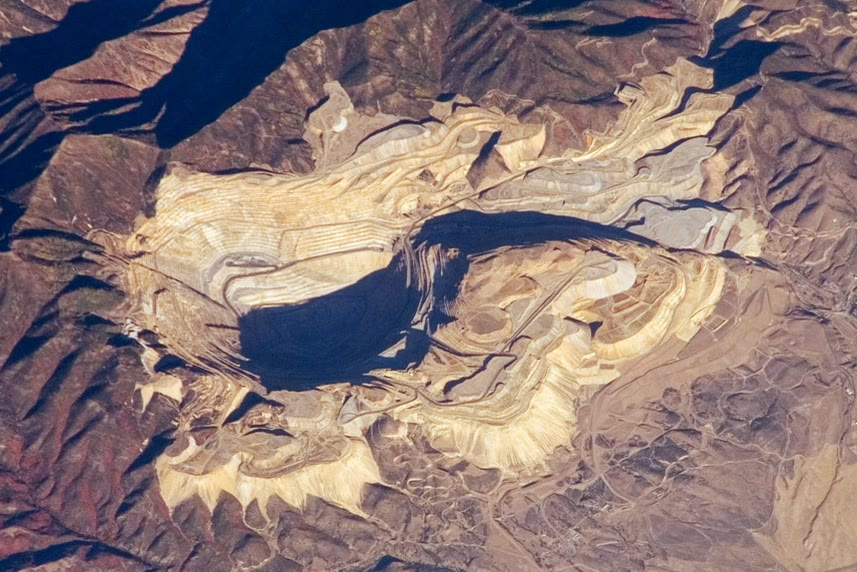
\includegraphics[width=0.5\linewidth]{images/book4/b2-29-bingham-canyon-iss.jpg}
\par\smallskip{\small 美国犹他州的 Bingham Canyon 露天矿坑，自国际空间站拍摄（2007 年）：
宽逾 \qty{4}{km}、深 \qty{1200}{m}，沿台阶开凿，台阶高 16 至 \qty{25}{m}，
开挖于\omterm{def:b2:ore-deposits:hydrothermal}{斑岩铜矿床}之中；周围平顶的丘陵为废石堆。照片：
NASA, Expedition 15 crew（公有领域）。}
\end{omfigure}
% ledger: photo:b2-29-bingham

\begin{definition}[矿床类型]\label{def:b2:ore-deposits:types}
\emph{矿床类型}\index{矿床类型}指一类\omterm{def:b2:ore-deposits:deposit}{矿床}，它们共享同一地质
环境、主岩、产出形态、矿石\omterm{def:b2:metamorphic-facies:assemblage}{矿物组合}与成矿过程，因而对该类的描述能够预测其成员的产出位置。
按成矿过程，这些类型分为四个族：
\omterm{def:b2:magma-emplacement:magma}{岩浆}型（金属在\omterm{def:b2:magma-emplacement:magma}{岩浆}结晶或分离时被富集），
热液型（由热的含水流体富集），沉积型（由沉积物的搬运与沉积，
或地表水中的沉淀作用），以及表生型（通过
早期\omterm{def:b2:ore-deposits:deposit}{矿床}的风化作用富集）。
\end{definition}

\section{岩浆型矿床}\label{sec:b2:ore-deposits:magmatic}

\textbf{\omterm{def:b2:magmatic-differentiation:cumulate}{层状侵入体}中的铬铁矿。}铬铁矿是唯一可商业利用的铬来源，
以块状铬铁岩层的形式富集，其中铬铁矿含量超过 \qty{90}{\percent}，位于超镁铁质
下部。侵入体宽 2 至 \qty{180}{km}，厚可达
\qty{15}{km}，矿层厚度自不足一厘米至 5--\qty{8}{m} 不等；它们共同
赋存了全球大部分铬储量，布什维尔德杂岩（已在
\cref{ch:b2:magmatic-differentiation}中介绍）是当今唯一开采铬铁矿的侵入体。其成因为堆晶层，
因\omterm{def:b2:magmatic-differentiation:open}{岩浆混合}或压力、
氧化态的改变而被推入铬铁矿相区，至今仍有争议。
% ledger: usgs10e:chromite

\textbf{镍–铜–铂族元素硫化物。}镁铁质或超镁铁质\omterm{def:b2:magma-emplacement:magma}{岩浆}，由大程度的
地幔熔融产生（\qty{20}{\percent} 至 \qty{25}{\percent} 或更高，MgO 含量按质量计超过 \qty{12}{\percent}），
上升时硫未饱和。若其同化地壳中的硫，或冷却得
足够充分，便达到饱和，不互溶的硫化物液体以液滴形式分离。
\omterm{def:b2:elements-in-the-earth:goldschmidt}{亲铜元素}进入这些液滴：比值 $D$ 为其在硫化物液体中的浓度
与硅酸盐液体中的浓度之比，即与矿物–熔体之间的分配系数同类，
其值对铜和镍为 $10^2$ 至 $10^3$，对
铂族元素为 $10^3$ 至 $10^4$。液滴能富集多少金属，取决于它遇到多少\omterm{def:b2:magma-emplacement:magma}{岩浆}。
% ledger: usgs10i:r-factor

\begin{proposition}[R 因子]\label{prop:b2:ore-deposits:r-factor}
设单位质量的硫化物液体与质量为 $R$ 的硅酸盐\omterm{def:b2:magma-emplacement:magma}{岩浆}在封闭体系中分离并达到平衡，
此质量比称为\emph{R 因子}\index{R 因子}；设 $C_L$ 为硫化物分离前\omterm{def:b2:magma-emplacement:magma}{岩浆}中某金属的浓度，
$D$ 为其硫化物–硅酸盐分配系数。则该金属在硫化物中的浓度为
系数。则该金属在硫化物中的浓度为
\begin{equation}
C_S = C_L\,\frac{D\,(R + 1)}{R + D} .
\label{eq:b2:ore-deposits:r-factor}
\end{equation}
当 $R \gg D$ 时，$C_S \to D\,C_L$；当 $R \ll D$ 时，$C_S \approx (R + 1)\,C_L$。
\end{proposition}

\begin{proof}
分离前，质量为 $R + 1$ 的体系含该金属 $(R + 1)C_L$。分离后，硅酸盐
中含 $R\,C_{\mathrm{sil}}$，硫化物中含 $C_S$，平衡时 $C_S = D\,C_{\mathrm{sil}}$。
由守恒得 $(R + 1)C_L = R\,C_S/D + C_S = C_S\,(R + D)/D$，于是
\eqref{eq:b2:ore-deposits:r-factor}。若 $R \gg D$，则 $(R + 1)/(R + D) \to 1$；若 $R \ll D$，
则 $D/(R + D) \to 1$。
\end{proof}

两个极限解释了为何存在两类硫化物矿石。当 $R \ll D$ 时，硫化物几乎
捕获所遇\omterm{def:b2:magma-emplacement:magma}{岩浆}中的全部金属，$C_S$ 随 $R$ 增大；当 $R \gg D$ 时，它
便达到饱和，其值为 $D\,C_L$，再多的\omterm{def:b2:magma-emplacement:magma}{岩浆}也无济于事。镍和铜的 $D$ 为数百，
在 $R$ 为数百至数千时达到上限，此即大多数镍–铜矿石的范围；
铂和钯的 $D$ 接近 $10^4$，含量持续增加，直至 $R$ 达到 \num{10000} 至
\num{100000}。富含铂族元素的矿石，如布什维尔德杂岩的 Merensky Reef 与
诺里尔斯克的部分矿石，因此记录了一小团硫化物被大质量的
\omterm{def:b2:magma-emplacement:magma}{岩浆}冲刷的过程（见练习~\ref{exo:b2:ore-deposits:5}和~\ref{exo:b2:ore-deposits:11}）。
% ledger: usgs10i:r-factor

\textbf{金伯利岩与金刚石。}大多数金刚石，以及几乎全部开采出的金刚石，形成于
厚大陆岩石圈的底部，即\omterm{def:b2:precambrian-earth:craton}{克拉通}的根部；金伯利\omterm{def:b2:magma-emplacement:magma}{岩浆}来自
深度超过 120 至 \qty{150}{km} 处，以高达 \qty{20}{m.s^{-1}} 的速度上升，将其携带至
地表，速度足够快，使其得以保存。金伯利岩优先穿过厚而老的岩石圈喷出，
这正是金刚石勘探的目标所在。
% ledger: grabreck22:kimberlite

\textbf{伟晶岩。}锂–铯–钽伟晶岩是富集这些稀有
元素的花岗质\omterm{def:b2:magma-emplacement:bodies}{岩墙}，形成于\omterm{def:b2:himalaya-andes:types}{碰撞造山带}中；其结晶温度约为 350 至 \qty{550}{\celsius}，
对花岗质熔体而言异常低，历时数日至数年，并长成巨大晶体——一颗
锂辉石晶体长 \qty{14}{m}。其锂矿物（锂辉石、透锂长石和
锂云母）约占全球锂供应的四分之一。
% ledger: usgs10o:lct

\section{热液型矿床}\label{sec:b2:ore-deposits:hydrothermal}

\begin{definition}[热液流体与热液型矿床类型]\label{def:b2:ore-deposits:hydrothermal}
\emph{热液流体}\index{热液流体}是一种热的含水流体，由\omterm{def:b2:magma-emplacement:magma}{岩浆}释放，
或由\omterm{def:b2:metamorphic-facies:reaction}{变质反应}产生，也可由加热的海水、大气降水或盆地卤水形成，它在流经岩石时溶解、
搬运并沉淀元素。热液型\omterm{def:b2:ore-deposits:deposit}{矿床}的主要类型
如下：
\begin{itemize}
  \item \emph{斑岩铜矿床}\index{斑岩铜矿床}：大型低品位矿体，
        由细脉与浸染状铜硫化物组成，赋存于小型斑岩株内及其周围，
        由\omterm{def:b2:magma-emplacement:magma}{岩浆}流体形成，位于俯冲带之上、地表以下数千米以内；
  \item \emph{浅成低温热液矿床}\index{浅成低温热液矿床}：金–银脉与
        浸染体，形成于地表以下约 \qty{1.5}{km} 范围内，温度约 100 至
        \qty{300}{\celsius}，产于火山弧中；
  \item \emph{火山成因块状硫化物矿床}\index{火山成因块状硫化物矿床}
        （VMS）：块状硫化物透镜体，形成于海底表面或其正下方，位于热液
        喷口处，产于海底火山环境中；
  \item \emph{沉积喷流矿床}\index{沉积喷流矿床}（sedex）：
        层状锌–铅硫化物，赋存于\omterm{def:b2:basins-compared:types}{裂谷盆地}的海相页岩中，沉淀于海底
        表面或其正下方，由沿断层上升的盆地卤水形成；
  \item \emph{密西西比河谷型矿床}\index{密西西比河谷型矿床}（MVT）：
        锌–铅硫化物置换台地碳酸盐岩，属后生成因，与火成活动无关，
        由盆地卤水沉淀形成；
  \item \emph{造山型金矿床}\index{造山型金矿床}：含金石英脉，产于
        变质带中，沿主要断层分布，由低盐度、富 CO$_2$ 的流体沉淀形成，
        其流体为变质成因。
\end{itemize}
\end{definition}
% ledger: usgs10b:form, usgs10q:epithermal, usgs10c:vms, usgs10n:sedex, usgs10a:mvt, drew03:orogenic

\textbf{搬运与沉淀。}大多数金属以配合物形式随\omterm{def:b2:ore-deposits:hydrothermal}{热液流体}搬运：
锌、铅和铜以氯配合物形式存在，因此盐度控制其溶解度；金则
在还原性流体中以硫配合物形式存在，例如 AuHS(H$_2$S)$_3$。当
溶解度下降时：流体冷却时；压强下降而沸腾时，逸出 H$_2$S 和 CO$_2$，并
使 pH 发生变化；与成分不同的流体混合时——卤水遇到富含
H$_2$S 的水，几乎立即沉淀出闪锌矿和方铅矿；流体与围岩反应时，
它会改变 pH 或氧化数。每一种\omterm{def:b2:ore-deposits:types}{矿床类型}，都是流体、
通道与圈闭的一种组合。
% ledger: usgs10n:sedex, drew03:orogenic

\textbf{斑岩铜矿。}斑岩\omterm{def:b2:ore-deposits:deposit}{矿床}提供了全球约 \qty{60}{\percent} 的
铜，并储有其约 \qty{65}{\percent} 的资源。它们以小型圆柱状
岩株或\omterm{def:b2:magma-emplacement:bodies}{岩墙}群为中心，也可以是较大\omterm{def:b2:magma-emplacement:bodies}{深成岩体}的顶部，侵位深度小于 5--\qty{10}{km}，
位于俯冲带之上的岛弧中，这正是\cref{ch:b2:magmatic-series}所述的环境。\omterm{def:b2:ore-deposits:deposit}{矿床}宽 0.1 至
\qty{1}{km}，高度相近；蚀变岩石可延伸至其周围 \qty{10}{km} 或更远。
随着\omterm{def:b2:magma-emplacement:magma}{岩浆}结晶，一种含盐量为 3 至 5 个百分比（按质量计）的流体从中分离出来；它上升、
减压后分裂为卤水和蒸气，两者都携带金属，而其超压
使岩石破裂。石英脉沉淀的温度约为 700 至 \qty{500}{\celsius}，而
流体与岩石的反应划分出蚀变带，详见下节。由于它们
形成于活动大陆边缘的浅部，那里剥蚀迅速，已知斑岩\omterm{def:b2:ore-deposits:deposit}{矿床}中超过 \qty{90}{\percent}
属新生代或中生代。
% ledger: usgs10b:share, usgs10b:form, usgs10b:fluids, usgs10b:alteration

\begin{omfigure}
\centering
\begin{tikzpicture}[x=1.15cm, y=1.15cm, font=\small]
\begin{scope}
\clip (-2.9,-3.6) rectangle (2.9,0);
% propylitic halo
\fill[omLithBasalt!45] (0,-1.25) ellipse (2.45 and 1.55);
% sodic-calcic deep flanks
\fill[omExo!25] (-1.75,-2.55) ellipse (0.45 and 0.38);
\fill[omExo!25] (1.75,-2.55) ellipse (0.45 and 0.38);
% sericitic shell
\fill[yellow!35] (0,-1.05) ellipse (1.15 and 1.15);
% potassic core
\fill[omProp!40] (0,-1.45) ellipse (0.68 and 0.85);
% ore shell
\draw[omThm, line width=1.1pt, densely dashed] (0,-1.3) ellipse (0.92 and 0.98);
% advanced argillic lithocap
\fill[omDef!30] (-1.05,0) .. controls (-0.6,-0.5) and (0.6,-0.5) .. (1.05,0) -- cycle;
\draw[omDef!70] (-1.05,0) .. controls (-0.6,-0.5) and (0.6,-0.5) .. (1.05,0);
\end{scope}
% pluton and stock
\fill[omLithGranite] (-2.6,-3.6) .. controls (-2.2,-2.9) and (-0.9,-2.6) .. (-0.3,-2.6)
  -- (-0.3,-1.25) arc[start angle=180, end angle=0, radius=0.3] -- (0.3,-2.6)
  .. controls (0.9,-2.6) and (2.2,-2.9) .. (2.6,-3.6) -- cycle;
\draw[black!60] (-2.6,-3.6) .. controls (-2.2,-2.9) and (-0.9,-2.6) .. (-0.3,-2.6)
  -- (-0.3,-1.25) arc[start angle=180, end angle=0, radius=0.3] -- (0.3,-2.6)
  .. controls (0.9,-2.6) and (2.2,-2.9) .. (2.6,-3.6);
% epithermal veins
\foreach \x in {1.45,1.65,1.85} \draw[omDef, line width=1pt] (\x,-0.02) -- (\x+0.12,-0.7);
% palaeosurface
\draw[black, line width=0.8pt] (-2.9,0) -- (2.9,0);
\node[anchor=south west, font=\scriptsize] at (-2.9,0) {古地表};
% labels
\draw[black!50] (0.6,-0.15) -- (1.2,0.25) -- (3.0,0.25) node[anchor=west, text=black] {高级泥化};
\draw[black!50] (1.95,-0.3) -- (3.0,-0.3) node[anchor=west, text=black] {浅成低温热液脉};
\draw[black!50] (1.05,-0.8) -- (3.0,-0.8) node[anchor=west, text=black] {绢云母化};
\draw[black!50] (0.85,-1.25) -- (3.0,-1.25) node[anchor=west, text=omThm] {铜矿壳};
\draw[black!50] (0.45,-1.7) -- (3.0,-1.7) node[anchor=west, text=black] {钾化};
\draw[black!50] (1.05,-2.15) -- (3.0,-2.15) node[anchor=west, text=black] {青磐岩化};
\draw[black!50] (2.1,-2.6) -- (3.0,-2.6) node[anchor=west, text=black] {钠–钙化};
\draw[black!50] (1.5,-3.15) -- (3.0,-3.15) node[anchor=west, text=black] {深成岩体与斑岩株};
\end{tikzpicture}
\par\smallskip{\small 斑岩铜矿系统剖面（示意图，未按比例）：核心为钾化带，
位于深部且温度高；向上、向外为绢云母化带，其中黄铁矿丰富；
两者之间为铜矿壳；周围为浅至中等深度的青磐岩化晕；
深部两翼为钠–钙化蚀变；上部为高级泥化帽；
在某些系统中，近地表处还有浅成低温热液脉。}
\end{omfigure}
% ledger: usgs10b:alteration

\textbf{浅成低温热液金矿。}在某些斑岩系统之上，以及一般而言在火山弧中，同类
流体会到达地壳上部 \qty{1.5}{km}，温度约为 100 至 \qty{300}{\celsius}，
在此处它们沸腾并与地下水混合；它们在石英脉中沉积金和银，伴随的
蚀变记录了近中性流体（冰长石、伊利石）或极酸性流体（高岭石、
迪开石、叶蜡石）的作用。
% ledger: usgs10q:epithermal, usgs10q:alteration

\textbf{海底块状硫化物。}海水下渗进入洋脊或
岛弧的热地壳，于约 \qty{350}{\celsius} 时以黑烟囱形式从喷口涌出，该现象
于 1979 年首次在东太平洋海隆被观测到。若喷口区持续活动，其硫化物便堆积成丘；矿石中
硫化物超过 \qty{40}{\percent}，其下方为标示供给通道的脉群网状体。金属
按温度分带：铁和铜位于高温底部，锌、铁、铅和钡位于较冷的顶部及
边缘，如下节所绘丘体所示。\omterm{def:b2:ore-deposits:hydrothermal}{火山成因块状硫化物
矿床}规模从不足一吨的透镜体，到西班牙里奥廷托的 \qty{1.5}{Gt}，并
年龄则从 \qty{3.55}{\Ga} 直到今日仍在形成的\omterm{def:b2:ore-deposits:deposit}{矿床}。
% ledger: usgs10c:vms

\textbf{盆地卤水：沉积喷流型与密西西比河谷型。}盆地卤水含溶解盐 \qty{10}{\percent} 至 \qty{30}{\percent}，
因埋藏而被加热至 100--\qty{200}{\celsius}，以氯配合物形式携带锌和铅，并形成
两种赋存于沉积物中的\omterm{def:b2:ore-deposits:types}{矿床类型}。沉积喷流型\omterm{def:b2:ore-deposits:deposit}{矿床}形成于卤水沿裂谷断层
喷入受限的还原性盆地，并与硫化氢相遇，形成层状硫化物泥的地方；它们占
全球锌和铅储量的一半以上。\omterm{def:b2:ore-deposits:hydrothermal}{密西西比河谷型矿床}形成于卤水被挤出
盆地、到达其边缘的碳酸盐台地，并在 75 至约
\qty{200}{\celsius} 下交代该台地；它们占沉积物中赋存的铅和锌\omterm{def:b2:ore-deposits:deposit}{矿床}的 \qty{38}{\percent}，
其中锌的含量约为铅的十倍。
% ledger: usgs10n:sedex, usgs10a:mvt

\textbf{造山型金矿。}在变质带中，\omterm{def:b2:metamorphic-facies:reaction}{脱挥发分反应}释放出近中性、
低盐度、富 CO$_2$ 的流体；沿主要断层导流，
于约 \qty{350}{\celsius} 及 4 至 \qty{12}{km} 深处沉淀出含金石英脉。这些脉体
沿很大高度连续延伸：印度科拉尔处达 \qty{3.2}{km}。
% ledger: drew03:orogenic

\section{沉积与表生矿床}\label{sec:b2:ore-deposits:sedimentary}

\begin{definition}[砂矿]\label{def:b2:ore-deposits:placer}
\emph{砂矿}\index{砂矿}是一种沉积\omterm{def:b2:ore-deposits:deposit}{矿床}，其中含密度大、性质稳定的矿物，
这些矿物由流动的水或风富集，因为在粒径相同时，它们比
周围的石英颗粒沉降更快，也更不易被携带。
\end{definition}

密度大于约 2.85 的矿物称为重矿物（石英为 2.65）：钛铁矿和锆石
约为 4.7，磁铁矿为 5.2，金为 15 至 19.3。由斯托克斯定律，颗粒的沉降速度随
超出密度 $\rho_s - \rho_w$ 增大，金的这一量为石英的十一倍，因此
同粒径的金与三倍粒径的石英沉降相当（见\cref{exo:b2:ore-deposits:3}）；金
通常留在基岩上的河流砾石中，而钛铁矿、金红石和锆石则到达海滩和
沙丘。重矿物砂的品位即重矿物的质量分数。
% ledger: usgs10l:heavy, usgs:gold-placer

化学沉积物同样是矿石。在\cref{ch:b2:precambrian-earth}中，\omterm{def:b2:precambrian-earth:bif}{条带状铁建造}
在海洋溶解铁被氧化时沉淀形成，是常见的铁矿石；蒸发岩
提供岩盐与钾盐；红土为深层热带风化的残余，
使铝富集，形成铝土矿。风化作用还会提高早先\omterm{def:b2:ore-deposits:deposit}{矿床}的品位。
% ledger: earle:bif, usgs:bauxite

\begin{definition}[表生富集，铁帽]\label{def:b2:ore-deposits:supergene}
\emph{表生富集}\index{表生富集}是金属在向下渗流的地下水作用下发生的富集：
在地下水位以上，含氧的酸性水从矿体的
硫化物中溶出金属；在其下方的还原条件下，金属又被沉淀，多以
置换原生硫化物。\emph{铁帽}\index{铁帽}是残留于地表的多孔、富含氧化铁的岩石，
覆于风化硫化矿体之上，其硫化物已被针铁矿、赤铁矿和
黄钾铁矾所取代。
\end{definition}

在斑岩\omterm{def:b2:ore-deposits:deposit}{矿床}中，地下水位以上的淋滤帽厚度可达
数百米；其下为富集的辉铜矿硫化物带，厚数十至数百米，
其铜品位为 0.4 至 \qty{1.7}{\percent}，总量超过 \qty{1.5}{Gt}，
始终富于其下的原生内生矿石。\omterm{def:b2:ore-deposits:supergene}{铁帽}与淋滤帽中的氧化铁保留了
被其取代的硫化物的结构，并指导下方的找矿；\omterm{def:b2:ore-deposits:supergene}{铁帽}及其铁染痕迹让早期矿工发现了许多
块状硫化物\omterm{def:b2:ore-deposits:deposit}{矿床}。
% ledger: usgs10b:supergene, usgs10c:vms

\begin{omfigure}
\centering
\begin{minipage}[b]{0.46\linewidth}\centering
\begin{tikzpicture}[x=1cm, y=1cm, font=\scriptsize]
\fill[omHist!55] (0,4.0) rectangle (1.8,5.2);
\fill[omMeth!30] (0,3.0) rectangle (1.8,4.0);
\fill[black!55] (0,1.8) rectangle (1.8,3.0);
\fill[black!18] (0,0) rectangle (1.8,1.8);
\draw (0,0) rectangle (1.8,5.2);
\draw[omDef, line width=1pt, densely dashed] (-0.25,3.0) -- (2.05,3.0);
\foreach \x in {0.45,0.9,1.35} \draw[omDef, -{Stealth[length=4pt]}] (\x,5.0) -- (\x,3.2);
\node[anchor=west, align=left] at (2.0,4.6) {铁帽与淋滤帽 \\（Fe 氧化物）};
\node[anchor=west, align=left] at (2.0,3.5) {氧化带 \\（孔雀石）};
\node[anchor=east, text=omDef, align=right] at (-0.25,3.0) {地下 \\水位};
\node[anchor=west, align=left] at (2.0,2.4) {富集层 \\（辉铜矿）};
\node[anchor=west, align=left] at (2.0,0.9) {原生矿石 \\（黄铜矿 \\+ 黄铁矿）};
\node[anchor=south, font=\scriptsize, text=omDef] at (0.9,5.25) {酸性水，Cu$^{2+}$};
\end{tikzpicture}
\end{minipage}\hfill
\begin{minipage}[b]{0.52\linewidth}\centering
\begin{tikzpicture}[x=1cm, y=1cm, font=\scriptsize]
\fill[omSea] (-2.6,1.4) rectangle (2.6,3.2);
\fill[omLithBasalt!60] (-2.6,-1.6) rectangle (2.6,1.4);
% stockwork cone
\fill[omProp!25] (-0.5,-1.6) -- (0.5,-1.6) -- (1.1,0.9) -- (-1.1,0.9) -- cycle;
\foreach \x/\y in {-0.3/-1.2,0.1/-1.0,-0.6/-0.4,0.4/-0.3,-0.1/0.1,0.6/0.4,-0.7/0.5}
  \draw[omProp!80!black] (\x,\y) -- ++(0.35,0.25);
% mound: upper rim and core
\fill[yellow!45] (-1.8,1.4) .. controls (-1.2,2.35) and (1.2,2.35) .. (1.8,1.4) -- cycle;
\fill[omThm!45] (-1.1,1.4) .. controls (-0.7,2.0) and (0.7,2.0) .. (1.1,1.4) -- cycle;
\draw (-1.8,1.4) .. controls (-1.2,2.35) and (1.2,2.35) .. (1.8,1.4);
% chimney and plume
\fill[black!70] (-0.08,2.1) rectangle (0.08,2.55);
\fill[black!45] (0,2.6) circle (0.12) (0.1,2.8) circle (0.16) (0.25,3.0) circle (0.2);
\draw[omDef, -{Stealth[length=4pt]}] (-2.3,2.9) -- (-2.3,0.2) -- (-1.2,-0.9);
\draw[omThm, -{Stealth[length=4pt]}] (0,-1.5) -- (0,1.2);
\node[anchor=west, text=omDef] at (-2.55,3.05) {海水};
\node[anchor=west] at (0.45,2.85) {黑烟囱，\qty{350}{\celsius}};
\draw[black!50] (1.45,1.75) -- (2.0,2.15) node[anchor=west, text=black] {Zn, Fe, Pb, Ba};
\draw[black!50] (0.6,1.6) -- (2.0,1.15) node[anchor=west, text=black] {Fe, Cu};
\node[anchor=west, align=left] at (0.95,-0.4) {网脉带 \\（供矿通道）};
\node[anchor=north, text=omThm] at (0,-1.6) {热流体};
\end{tikzpicture}
\end{minipage}
\par\smallskip{\small 左：覆于铜硫化物矿体之上的表生剖面（示意图，非按比例
）：酸性水在地下水位以上淋滤铜，并在其下以辉铜矿形式再沉淀，
在地表留下\omterm{def:b2:ore-deposits:supergene}{铁帽}。右：火山成因块状硫化物丘的剖面（示意
图）：海水在地壳中受热，沿网脉带上升，以黑烟囱形式喷出；矿丘呈
分带：底部为热区，富铁、铜，顶部和
边缘富锌、铁、铅和钡。}
\end{omfigure}
% ledger: usgs10b:supergene, usgs10c:vms

\begin{omfigure}
\centering
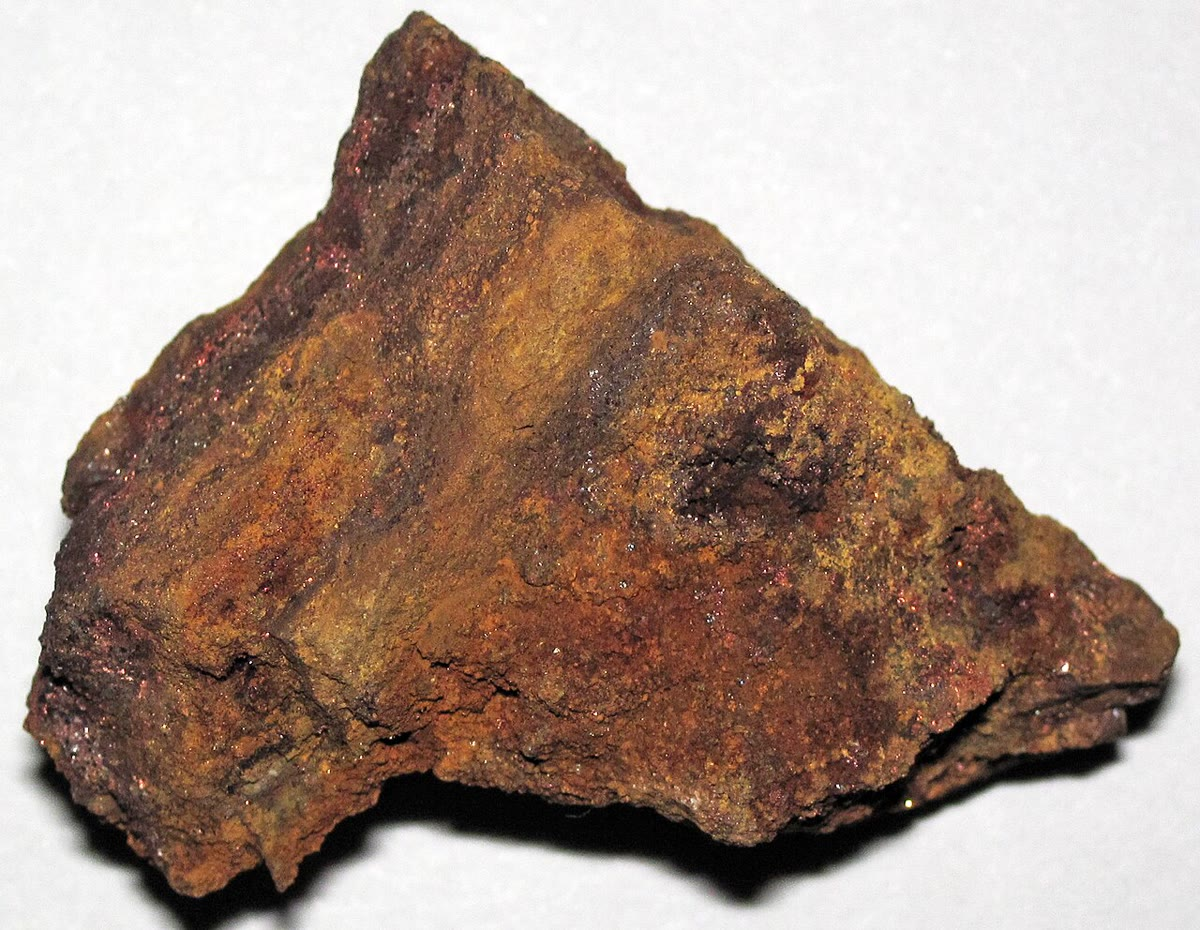
\includegraphics[width=0.4\linewidth]{images/book4/b2-29-flambeau-gossan.jpg}
\par\smallskip{\small 威斯康星州 Flambeau 块状硫化物\omterm{def:b2:ore-deposits:deposit}{矿床}的\omterm{def:b2:ore-deposits:supergene}{铁帽}：一种多孔岩石，
由黄铁矿、黄铜矿、辉铜矿和斑铜矿风化残留的含铁羟基氧化物构成，
形成于古元古代火山弧中；小橙色斑点为自然铜。照片：James St.
John（CC BY 2.0）。}
\end{omfigure}
% ledger: photo:b2-29-gossan

\section{品位与吨位}\label{sec:b2:ore-deposits:grade-tonnage}

一份世界汇编列出了 422 个\omterm{def:b2:ore-deposits:hydrothermal}{斑岩铜矿床}的吨位，按可得的最低
\omterm{def:b2:ore-deposits:grade}{边界品位}计算，并列出其平均铜品位。其中十分之一超过 \qty{1500}{Mt}，十分之一
少于 \qty{33}{Mt}，中位数为 \qty{240}{Mt}；品位在相同十分位数之间从 \qty{0.24}{\percent} 变至
\qty{0.75}{\percent}，中位数为 \qty{0.44}{\percent}。
十分位数之间吨位跨越 45 倍，品位跨越 3 倍。在对数坐标下两张直方图均接近正态曲线，如下图所示：
吨位对数的均值为 2.373，标准差为 0.654，品位的对数
均值为 $-0.364$，标准差为 0.199（对数以 10 为底，吨位以百万吨计，品位以百分数计）。拟合
并不理想：品位比对数正态律更尖锐，少数品位极低的\omterm{def:b2:ore-deposits:deposit}{矿床}使其
在正式检验中偏离该律。二者几乎独立，
其对数之间的相关系数为 0.1。
% ledger: usgs08:table1, usgs08:independence, data:b4-porphyry-cu

\begin{omfigure}
\centering
\begin{minipage}[b]{0.49\linewidth}\centering
\begin{tikzpicture}
\begin{axis}[omrecord, width=0.96\linewidth, height=4.5cm, xmin=0.5, xmax=5.0, ymin=0, ymax=80,
  xlabel={吨位（Mt）}, ylabel={矿床数目},
  xtick={1,2,3,4,5}, xticklabels={10,100,1000,$10^4$,$10^5$},
  tick label style={font=\scriptsize}, label style={font=\small}]
% computed in figdata/bachelor-2/ores.py part hist_t; ledger: data:b4-porphyry-cu
\addplot[ybar, bar width=0.22, fill=omDef!35, draw=omDef!70] table[x=log10_t, y=count] {figdata/out/bachelor-2-ores-hist_t.dat};
\addplot[omThm, line width=1pt, smooth] table[x=log10_t, y=fit] {figdata/out/bachelor-2-ores-hist_t.dat};
\end{axis}
\end{tikzpicture}
\end{minipage}\hfill
\begin{minipage}[b]{0.49\linewidth}\centering
\begin{tikzpicture}
\begin{axis}[omrecord, width=0.96\linewidth, height=4.5cm, xmin=-1.2, xmax=0.6, ymin=0, ymax=120,
  xlabel={铜品位（\%）}, ylabel={矿床数目},
  xtick={-1,-0.69897,-0.30103,0,0.30103}, xticklabels={0.1,0.2,0.5,1,2},
  tick label style={font=\scriptsize}, label style={font=\small}]
% computed in figdata/bachelor-2/ores.py part hist_g; ledger: data:b4-porphyry-cu
\addplot[ybar, bar width=0.088, fill=omDef!35, draw=omDef!70] table[x=log10_g, y=count] {figdata/out/bachelor-2-ores-hist_g.dat};
\addplot[omThm, line width=1pt, smooth] table[x=log10_g, y=fit] {figdata/out/bachelor-2-ores-hist_g.dat};
\end{axis}
\end{tikzpicture}
\end{minipage}
\par\smallskip{\small 全球汇编中 422 个\omterm{def:b2:ore-deposits:hydrothermal}{斑岩铜矿床}的吨位（左）与铜品位（右），
均以对数坐标绘制，红色曲线为具有相同均值和标准差的正态曲线。
数据来源：Singer, Berger and Moring（2008），USGS。}
\end{omfigure}

\begin{proposition}[对数正态变量之积]\label{prop:b2:ore-deposits:product}
若 $\log_{10} T$ 与 $\log_{10} g$ 联合正态，均值分别为 $\mu_T$ 和 $\mu_g$，标准差
分别为 $\sigma_T$ 和 $\sigma_g$，相关系数为 $\rho$，则所含金属量 $M = Tg/100$
（$g$ 以百分数计）服从对数正态分布，即 $\log_{10} M$ 服从正态分布，且
\begin{equation}
\mu_M = \mu_T + \mu_g - 2 , \qquad
\sigma_M^2 = \sigma_T^2 + \sigma_g^2 + 2\rho\,\sigma_T\sigma_g .
\label{eq:b2:ore-deposits:product}
\end{equation}
\end{proposition}

\begin{proof}
$\log_{10} M = \log_{10} T + \log_{10} g - 2$。联合正态变量的线性组合
仍服从正态分布（此结论取自数学教材，在本阶段不加证明地承认）；其均值为各均值之和，
其方差 $\operatorname{var}(X + Y) = \operatorname{var} X + \operatorname{var} Y + 2\operatorname{cov}(X, Y)$，
其中 $\operatorname{cov}(X, Y) = \rho\,\sigma_T\sigma_g$。
\end{proof}

对斑岩\omterm{def:b2:ore-deposits:deposit}{矿床}，$\sigma_M = \sqrt{0.654^2 + 0.199^2 + 2 \times 0.1 \times 0.654 \times
0.199} = 0.702$，$\mu_M = 0.009$：中位\omterm{def:b2:ore-deposits:deposit}{矿床}约含 \qty{1}{Mt} 铜，所含金属的分散程度
甚至比吨位更大。对数正态分布若离散如此之大，则大部分金属集中于少数\omterm{def:b2:ore-deposits:deposit}{矿床}：最大的
十分之一\omterm{def:b2:ore-deposits:deposit}{矿床}按该定律约含 \qty{63}{\percent} 的
铜，数据中为 \qty{64}{\percent}（见练习~\ref{exo:b2:ore-deposits:12}）。下图按吨位与品位标出每个\omterm{def:b2:ore-deposits:deposit}{矿床}，
并画出等含铜量线；
宾厄姆\omterm{def:b2:ore-deposits:deposit}{矿床}（吨位 \qty{28.5}{Mt}）位于 10 与 \qty{100}{Mt} 两条线之间。
% ledger: data:b4-porphyry-cu
% values: sd_log10_m 0.702233, mean 0.00857; median M 1.02 Mt; top 10 % share 0.631 (fit) 0.643 (data)

\begin{definition}[品位–吨位曲线]\label{def:b2:ore-deposits:gt}
\omterm{def:b2:ore-deposits:deposit}{矿床}的\emph{品位–吨位曲线}\index{品位–吨位曲线}给出，
以截止品位 $c$ 为自变量的函数：吨位 $T(c)$（即品位高于 $c$ 的块体的吨位）及其平均品位
$\bar g(c)$。
\end{definition}

\begin{proposition}[对数正态矿床的品位–吨位曲线]\label{prop:b2:ore-deposits:gt}
若总吨位为 $T_0$ 的\omterm{def:b2:ore-deposits:deposit}{矿床}中各块体的品位服从对数正态分布，即 $\ln g$ 服从正态分布，
其均值为 $\mu$（中位品位为 $e^{\mu}$），标准差为 $s$，记 $z = (\mu -
\ln c)/s$，则有
\begin{equation}
T(c) = T_0\,\Phi(z), \qquad
\bar g(c) = e^{\mu + s^2/2}\,\frac{\Phi(z + s)}{\Phi(z)} ,
\label{eq:b2:ore-deposits:gt}
\end{equation}
截止品位以上的金属量为 $M(c) = T_0\,e^{\mu + s^2/2}\,\Phi(z + s)$，占总量的 $\Phi(z +
s)$。
\end{proposition}

\begin{proof}
记 $\ln g = \mu + s u$，$u$ 为标准正态变量。块体高于截止品位，当 $u > (\ln c -
\mu)/s = -z$ 时，其概率为 $1 - \Phi(-z) = \Phi(z)$，故得 $T(c)$。截止品位以上的金属量
（按单位总吨位计）为 $\int_{-z}^{\infty} e^{\mu + s u}\,\varphi(u)\,\mathrm{d}u$，
其中 $\varphi$ 为标准正态密度。配方得 $e^{su}\varphi(u) =
e^{s^2/2}\varphi(u - s)$，故积分为 $e^{\mu + s^2/2}\,[1 - \Phi(-z - s)] = e^{\mu +
s^2/2}\,\Phi(z + s)$。除以 $\Phi(z)$ 即得平均品位。
\end{proof}

当 $c \to 0$ 时整个\omterm{def:b2:ore-deposits:deposit}{矿床}被保留，其平均品位为 $e^{\mu + s^2/2}$，高于
中位品位。提高截止品位所去掉的吨位比金属量下降得更快，因为被去掉的是
最贫的块体。以图中示意\omterm{def:b2:ore-deposits:deposit}{矿床}为例，将截止品位由 0.2 提高到
\qty{0.5}{\percent} 时，仅保留 \qty{41}{\percent} 的吨位，却保留了 \qty{61}{\percent} 的铜。
% values: demo T 876.0/355.0 Mt, M 4.599/2.826 Mt (figdata ores.py gtcurve)

\begin{omfigure}
\centering
\begin{minipage}[b]{0.49\linewidth}\centering
\begin{tikzpicture}
\begin{axis}[omrecord, width=0.96\linewidth, height=5.0cm, xmode=log, ymode=log,
  xmin=2, xmax=50000, ymin=0.05, ymax=2.8, xlabel={吨位 (Mt)}, ylabel={铜品位 (\%)},
  ytick={0.1,0.2,0.5,1,2}, yticklabels={0.1,0.2,0.5,1,2},
  tick label style={font=\scriptsize}, label style={font=\small}]
% computed in figdata/bachelor-2/ores.py parts scatter and iso; ledger: data:b4-porphyry-cu
\addplot[black!45, line width=0.6pt, unbounded coords=jump] table[x=tonnage_mt, y=g01] {figdata/out/bachelor-2-ores-iso.dat};
\addplot[black!45, line width=0.6pt, unbounded coords=jump] table[x=tonnage_mt, y=g1] {figdata/out/bachelor-2-ores-iso.dat};
\addplot[black!45, line width=0.6pt, unbounded coords=jump] table[x=tonnage_mt, y=g10] {figdata/out/bachelor-2-ores-iso.dat};
\addplot[black!45, line width=0.6pt, unbounded coords=jump] table[x=tonnage_mt, y=g100] {figdata/out/bachelor-2-ores-iso.dat};
\addplot[omDef, only marks, mark=*, mark size=0.8pt, opacity=0.7] table[x=tonnage_mt, y=cu_pct] {figdata/out/bachelor-2-ores-scatter.dat};
\addplot[omThm, only marks, mark=square*, mark size=2pt] coordinates {(3230,0.882)};
\node[font=\tiny, text=black!70, fill=white, inner sep=1pt] at (axis cs:4.55,2.2) {0.1};
\node[font=\tiny, text=black!70, fill=white, inner sep=1pt] at (axis cs:45.5,2.2) {1};
\node[font=\tiny, text=black!70, fill=white, inner sep=1pt] at (axis cs:455,2.2) {10};
\node[font=\tiny, text=black!70, fill=white, inner sep=1pt] at (axis cs:4545,2.2) {100 Mt};
\node[font=\scriptsize, text=omThm, anchor=south, fill=white, inner sep=1pt] at (axis cs:3230,1.0) {宾厄姆};
\end{axis}
\end{tikzpicture}
\end{minipage}\hfill
\begin{minipage}[b]{0.49\linewidth}\centering
\begin{tikzpicture}
\begin{axis}[omrecord, width=0.80\linewidth, height=5.0cm, xmin=0, xmax=1.2, ymin=0, ymax=1000,
  xlabel={截止品位 (\%)}, ylabel={高于截止品位的吨位 (Mt)}, axis y line*=left,
  ylabel style={text=omDef}, tick label style={font=\scriptsize}, label style={font=\small}]
% computed in figdata/bachelor-2/ores.py part gtcurve (illustrative deposit)
\addplot[omDef, line width=1.1pt] table[x=cutoff_pct, y=tonnage_mt] {figdata/out/bachelor-2-ores-gtcurve.dat};
\end{axis}
\begin{axis}[width=0.80\linewidth, height=5.0cm, xmin=0, xmax=1.2, ymin=0, ymax=1.6,
  axis y line*=right, axis x line=none, ylabel={高于截止品位的平均品位 (\%)},
  ylabel style={text=omThm}, tick label style={font=\scriptsize}, label style={font=\small}]
\addplot[omThm, line width=1.1pt, densely dashed] table[x=cutoff_pct, y=grade_pct] {figdata/out/bachelor-2-ores-gtcurve.dat};
\end{axis}
\end{tikzpicture}
\end{minipage}
\par\smallskip{\small 左图：422 个\omterm{def:b2:ore-deposits:hydrothermal}{斑岩铜矿床}的吨位与铜品位，并附等含铜量线
（0.1 至 \qty{100}{Mt}）；红色方块为宾厄姆峡谷矿。数据来源：
Singer, Berger and Moring（2008），USGS。右图为示意\omterm{def:b2:ore-deposits:deposit}{矿床}的\omterm{def:b2:ore-deposits:gt}{品位–吨位曲线}，
总吨位 \qty{1000}{Mt}，中位品位 \qty{0.40}{\percent}，$s = 0.60$：截止品位以上的吨位（蓝色）
及其平均品位（红色虚线），由 \eqref{eq:b2:ore-deposits:gt} 得出。}
\end{omfigure}

\section{勘查}\label{sec:b2:ore-deposits:exploration}

\omterm{def:b2:ore-deposits:deposit}{矿床}多通过其矿石之外留下的痕迹而被发现。斑岩系统的蚀变晕
宽以千米计，在岩石出露处，其矿物可由航空器
和卫星依其红外光谱进行填图；其金属元素扩散入周围的
土壤、水系沉积物、水体和植物中；其硫化物与蚀变岩会改变地球物理探测所测量的物理性质。
% ledger: usgs10b:form, usgs10b:exploration, usgs10b:remote

\begin{definition}[地球化学异常]\label{def:b2:ore-deposits:exploration}
称\emph{地球化学异常}\index{地球化学异常}为某一元素或某组元素
在取样介质——岩石、土壤、河流沉积物、水体、植物——中的浓度，
它偏离该区域的背景值，即在不存在矿化作用的地方所见的
浓度范围。
\end{definition}

与品位相似，浓度跨越若干数量级，因此异常通常依据
对数进行判断；练习~\ref{exo:b2:ore-deposits:9} 中所用的一个简单阈值，取为
背景对数值的均值加上其标准差的两倍。河流沉积物样品
混合了整个汇水区的沉积物，因此异常沿下游方向减弱，干净的沉积物不断汇入其中，
浓度梯度则指向流域上游的源头。在覆盖于
埋藏伟晶岩之上的土壤中，锂、铷、铯、钽和锡的异常已被追踪到
未出露的岩体上方。
% ledger: usgs10b:exploration, usgs10o:lct

地球物理方法的选择取决于\omterm{def:b2:ore-deposits:types}{矿床类型}所提供的对比度。浸染状硫化物使
岩石起到电容器的作用：测量这一充电率的激发极化法，
最初是为斑岩铜矿发展的，它对富黄铁矿的绢云母化带响应最强，钾化
核心的硫化物较少。磁法与重力测量用于圈定与\omterm{def:b2:ore-deposits:deposit}{矿床}相关的\omterm{def:b2:magma-emplacement:bodies}{深成岩体}。
没有任何方法能直接探测矿石，
在钻孔加以检验之前，每种解释都是非唯一的。
% ledger: usgs10b:exploration

\begin{method}[由化验结果到资源量估算]\label{met:b2:ore-deposits:resource}
数据来自沿网格布设于\omterm{def:b2:ore-deposits:deposit}{矿床}上方的钻孔，岩芯经编录后按
已知长度的区段进行化验。
\begin{enumerate}
  \item \textbf{组合样。} 按等长对化验结果取平均，每个化验值以其长度加权，
        使每个组合样代表相同的体积。
  \item \textbf{建模。} 将\omterm{def:b2:ore-deposits:deposit}{矿床}划分为块体，由邻近的组合样估算每个块体的品位，
        并按距离及品位的空间相关性确定权重，
        （地质统计方法克里金法，在本阶段不加证明地承认）。
  \item \textbf{报告。} 施加\omterm{def:b2:ore-deposits:grade}{边界品位}，在钻孔间距所允许的每个置信水平下，
        给出高于\omterm{def:b2:ore-deposits:grade}{边界品位}的块体的\omterm{def:b2:ore-deposits:grade}{矿石量}、平均品位及岩石密度。
\end{enumerate}
\end{method}

\begin{inthefield}[编录钻孔岩芯]
\centering
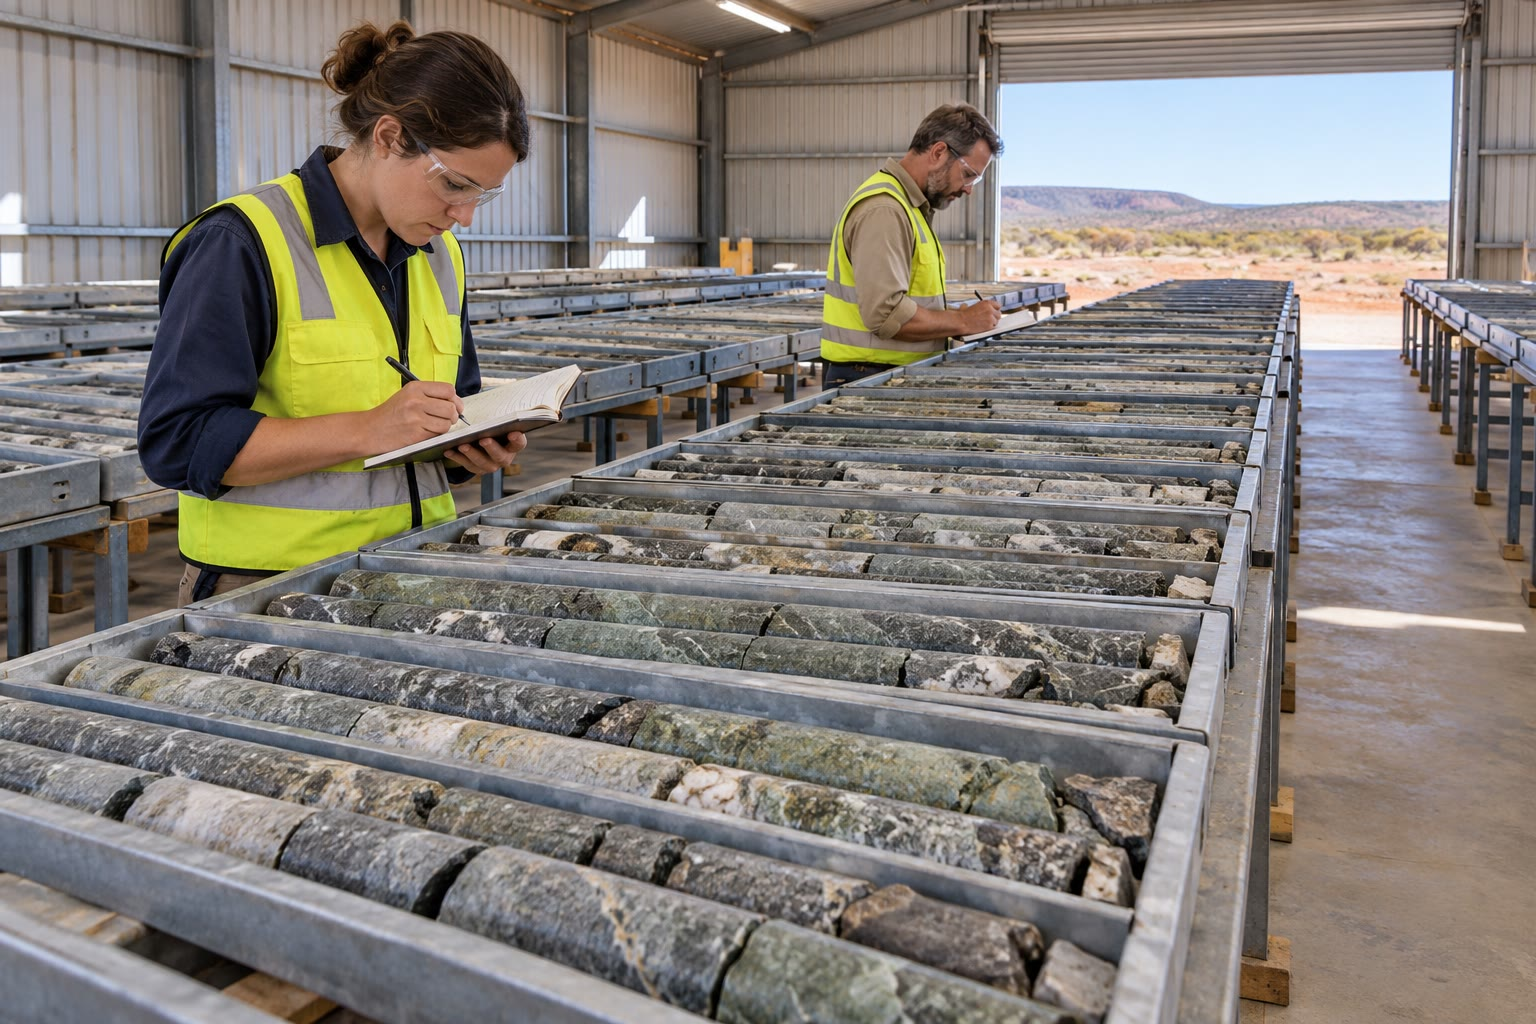
\includegraphics[width=0.56\linewidth]{images/book4/ai/b2-core-shed.jpg}
\par\smallskip{\small 勘探项目中的岩芯库（AI 生成的插图）。}
\par\medskip\raggedright
在勘探项目中，每个钻孔的岩芯按其自地下取出的顺序，
摆放于金属托盘中。地质人员沿托盘逐段查看，记录
岩石的类型、蚀变情况、切穿它的矿脉及其所占比例，以及其中所含的硫化物；
并标出岩芯将被锯开取样的位置。编录先于化验，并与化验结果相互比照：
携带金属的蚀变带或矿脉类型，便成为需要逐孔追踪的对象，
从一个钻孔追踪到另一个钻孔；地质人员再据编录资料绘制剖面，
据此规划下一批钻孔。
\end{inthefield}

\section*{练习}\label{sec:b2:ore-deposits:exercises}

除非另有说明，练习所用数据如下：上陆壳中铜 \qty{28}{ppm}，
金 \qty{1.5}{ng/g}、铬 \qty{92}{ppm}；斑岩铜矿总体见
\cref{sec:b2:ore-deposits:grade-tonnage}，$\log_{10}$ 吨位（Mt）的均值为 2.373，标准
差为 0.654，$\log_{10}$ 品位（\%）的均值为 $-0.364$，标准差为 0.199，相关系数
$\rho = 0.100$。结果保留三位有效数字。
% ledger: rg03:ucc-trace, data:b4-porphyry-cu

\begin{exercise}[$\star$]\label{exo:b2:ore-deposits:1}
求下列矿石相对于上陆壳的\omterm{def:b2:ore-deposits:cf}{富集系数}：(a) 铜矿石，
品位为 \qty{0.5}{\percent}；(b) 金矿石，品位为 \qty{6}{g/t}；(c) 含铬铁矿 \qty{90}{\percent} 的铬铁岩，
取铬铁矿为 FeCr$_2$O$_4$（原子量 Cr 52.00、Fe 55.85、O 16.00）。
\end{exercise}

\begin{exercise}[$\star$]\label{exo:b2:ore-deposits:2}
Batu Hijau 报告如下：在\omterm{def:b2:ore-deposits:grade}{边界品位} \qty{0.3}{\percent} 以上，矿量 \qty{914}{Mt}，Cu 品位 \qty{0.53}{\percent}，Au 品位 \qty{0.40}{g/t}；
在最低可取\omterm{def:b2:ore-deposits:grade}{边界品位}下，矿量 \qty{1640}{Mt}，Cu 品位 \qty{0.44}{\percent}，
Au 品位 \qty{0.45}{g/t}。(a) 求每个估算所含的铜（Mt）与金（t）。
(b) 第二个估算中多出的块体增加了多少矿量和多少铜，
其平均品位为多少？(c) 为什么两个估算都是正确的？
\end{exercise}

\begin{exercise}[$\star$]\label{exo:b2:ore-deposits:3}
在斯托克斯定律中，直径为 $d$ 的颗粒的沉降速度与 $(\rho_s -
\rho_w)\,d^2$ 成正比。取 $\rho_w = 1.00$，石英 2.65，金 19.3，锆石 4.7（单位为
\unit{g.cm^{-3}}）。(a) 同样大小时，金颗粒比石英颗粒沉降快多少倍？
(b) 沉降速度相同的金颗粒与石英颗粒，其直径之比为多少？
(c) 哪种石英颗粒的沉降情况与 \qty{0.1}{mm} 的锆石颗粒相同？
\end{exercise}

\begin{exercise}[$\star$]\label{exo:b2:ore-deposits:4}
一块原生铜矿的品位为 \qty{0.4}{\percent}。风化作用将其全部铜淋滤，
作用厚度为 \qty{150}{m}，并在其正下方重新沉淀于厚 \qty{50}{m} 的富集层中，
两者密度相同。(a) 求该富集层的品位。(b) 若只有 \qty{80}{\percent} 的
淋滤铜被重新沉淀，结果如何？(c) 若淋滤铜全部重新沉淀，淋滤层厚度为多少时，
富集层品位为 \qty{1.7}{\percent}？
\end{exercise}

\begin{exercise}[$\star\star$]\label{exo:b2:ore-deposits:5}
某\omterm{def:b2:magma-emplacement:magma}{岩浆}中含铂 \qty{10}{ppb}、镍 \qty{200}{ppm}；取 $D_{\mathrm{Pt}} =
10^4$，$D_{\mathrm{Ni}} = 500$。(a) 利用 \eqref{eq:b2:ore-deposits:r-factor}，求
硫化物中铂（ppm）与镍（wt\%）的含量，取 $R = 100$、\num{1000}、\num{10000}
及 \num{100000}。(b) 求 $R \to \infty$ 时它们的极限。(c) 解释为何镍矿石
很少能说明 $R$，而铂矿石则能说明很多。
\end{exercise}

\begin{exercise}[$\star\star$]\label{exo:b2:ore-deposits:6}
利用 \eqref{eq:b2:ore-deposits:product} 处理斑岩铜矿总体：(a) 求 $\log_{10} M$ 的均值与
标准差，以及所含铜的中位数。(b) 含铜量超过 \qty{10}{Mt} 的\omterm{def:b2:ore-deposits:deposit}{矿床}
所占比例为多少？在 422 个\omterm{def:b2:ore-deposits:deposit}{矿床}中有多少个？(c) 忽略相关性，重做 (b)。
\end{exercise}

\begin{exercise}[$\star\star$]\label{exo:b2:ore-deposits:7}
对图中的示意\omterm{def:b2:ore-deposits:deposit}{矿床}（$T_0 = \qty{1000}{Mt}$，中位品位 \qty{0.40}{\percent}，
$s = 0.60$），利用 \eqref{eq:b2:ore-deposits:gt}，求高于\omterm{def:b2:ore-deposits:grade}{边界品位} \qty{0.3}{\percent} 与
\qty{0.6}{\percent} 的矿量、平均品位与所含铜量。并在图上核对其中一点。
\end{exercise}

\begin{exercise}[$\star\star$]\label{exo:b2:ore-deposits:8}
一座斑岩\omterm{def:b2:ore-deposits:deposit}{矿床}含铜 \qty{5}{Mt}。设其\omterm{def:b2:magma-emplacement:magma}{岩浆}流体携带 \qty{1000}{ppm} 的铜，
其中一半沉积于矿石中，并设\omterm{def:b2:magma-emplacement:magma}{岩浆}释放出其质量的 \qty{3.5}{\percent}
作为流体。(a) 求所需流体与\omterm{def:b2:magma-emplacement:magma}{岩浆}的质量。(b) 求\omterm{def:b2:magma-emplacement:magma}{岩浆}的
体积，\omterm{def:b2:magma-emplacement:magma}{岩浆}密度为 \qty{2600}{kg.m^{-3}}。(c) 若\omterm{def:b2:magma-emplacement:magma}{岩浆}含铜 \qty{50}{ppm}，则其中
有多大比例最终进入了矿石？
\end{exercise}

\begin{exercise}[$\star\star$]\label{exo:b2:ore-deposits:9}
八个背景河流沉积物的 $\log_{10}$ Cu（ppm）值分别为 1.30、1.45、1.38、1.52、1.41、1.35、
1.48 与 1.40。(a) 求这些对数值的均值与标准差（总体标准差）、背景中位数，
以及以 ppm 计的阈值（均值加两倍标准差）。(b) 一条支流
汇水区面积为 \qty{4}{km^2}，流经矿化地表，其沉积物含量为 \qty{400}{ppm}；它汇入一条
汇水区面积为 \qty{36}{km^2}、沉积物含量为背景中位数的河流。假设每平方千米提供相同质量的沉积物，
则混合沉积物是否异常？(c) 汇水区总面积至多为多大时，
异常仍高于阈值？
\end{exercise}

\begin{exercise}[$\star\star\star$]\label{exo:b2:ore-deposits:10}
(a) 证明 $e^{su}\varphi(u) = e^{s^2/2}\varphi(u - s)$。(b) 由此推出对数正态
变量的均值 $e^{\mu + s^2/2}$。(c) 证明高于\omterm{def:b2:ore-deposits:grade}{边界品位}的金属比例
$\Phi(z + s)$ 总大于矿量比例 $\Phi(z)$，并说明其含义。
\end{exercise}

\begin{exercise}[$\star\star\star$]\label{exo:b2:ore-deposits:11}
(a) 由 \eqref{eq:b2:ore-deposits:r-factor}，求 $R$，使 $C_S$ 达到某一比例 $f$
（相对于上限 $D\,C_L$）时所对应的值。(b) 取 $f = 0.5$ 与 $0.9$，并取 $D = 300$（镍）与 $D =
10^4$（铂），计算其值。(c) 与文中给出的镍–铜矿石及铂族元素礁的 $R$ 取值范围
进行比较。
\end{exercise}

\begin{exercise}[$\star\star\star$]\label{exo:b2:ore-deposits:12}
(a) 设对数正态变量 $M$，其 $\ln M$ 的标准差为 $s$，证明高于
$q$ 阶分位数的\omterm{def:b2:ore-deposits:deposit}{矿床}占总金属量的比例为 $\Phi\bigl(s - \Phi^{-1}(q)\bigr)$。
(b) 对斑岩\omterm{def:b2:ore-deposits:deposit}{矿床}总体，取 $q = 0.9$，计算该比例。(c) 对 $q = 0.99$ 做同样的计算，并与
汇编中四个最大\omterm{def:b2:ore-deposits:deposit}{矿床}相比较，它们占汇编铜量的 \qty{26.6}{\percent}。
\end{exercise}
% ledger: data:b4-porphyry-cu

\begin{problem}[{周末问题——一处斑岩勘探区}]\label{pb:b2:ore-deposits:1}
一处斑岩勘探区（虚构）已被钻探。其发现孔共切穿八段，自上而下
（长度以米计，铜品位以百分比计）：30 米，0.12；40 米，0.35；50 米，0.62；60
米，0.48；40 米，0.27；30 米，0.81；50 米，0.41；30 米，0.18。全部钻孔的地质统计研究表明
块段品位服从对数正态分布，中位数为 \qty{0.38}{\percent}，$s = 0.55$
为 $\ln g$ 的标准差。矿化体接近竖直圆柱体，半径为 \qty{450}{m}、
高为 \qty{700}{m}，密度为 \qty{2.7}{t.m^{-3}}。利用各练习的数据，结果保留三位
有效数字（概率保留四位）。

\noindent\textbf{第一部分——发现孔。}
\begin{enumerate}
  \item 求所取样段的长度及其按长度加权的平均品位。
  \item 求八个品位的算术平均值。为何加权平均才是正确的？
  \item 长度中有多大比例高于 \qty{0.3}{\percent}，其平均品位为多少？
  \item 求加权平均品位相对上地壳的\omterm{def:b2:ore-deposits:cf}{富集系数}。
  \item 对最富的一段做同样的计算。
  \item 求\omterm{def:b2:ore-deposits:deposit}{矿床}全部块段的平均品位。发现孔是否具有代表性？
\end{enumerate}

\noindent\textbf{第二部分——\omterm{def:b2:ore-deposits:grade}{边界品位}以上的矿量。}
\begin{enumerate}[resume]
  \item 求矿体的体积及矿量 $T_0$；取 $T_0 = \qty{1200}{Mt}$。
  \item 对于\omterm{def:b2:ore-deposits:grade}{边界品位} \qty{0.3}{\percent}，求 $z$ 及高于该品位的块段比例。
  \item 求高于\omterm{def:b2:ore-deposits:grade}{边界品位} 0.2、0.3 与 \qty{0.5}{\percent} 的矿量。
  \item 求高于 \qty{0.3}{\percent} \omterm{def:b2:ore-deposits:grade}{边界品位}的平均品位。
  \item 对 0.2 与 \qty{0.5}{\percent} 做同样的计算。
  \item 将\omterm{def:b2:ore-deposits:grade}{边界品位}由 0.3 提高到 \qty{0.5}{\percent}：矿量与
        平均品位各变为原来的多少倍？
  \item 保留一半矿量时对应的\omterm{def:b2:ore-deposits:grade}{边界品位}为多少？其平均品位是多少？
\end{enumerate}

\noindent\textbf{第三部分——该勘探区在全球斑岩\omterm{def:b2:ore-deposits:deposit}{矿床}中的位置。}
\begin{enumerate}[resume]
  \item 求整个矿体按平均品位计算所含的铜量。
  \item 求其矿量在全球总体中的标准分数及其百分位。
  \item 对其平均品位做同样的计算。
  \item 求考虑相关性与不考虑相关性时 $\log_{10} M$ 的标准差。
  \item 求其所含铜量的百分位。
  \item 在 422 个\omterm{def:b2:ore-deposits:deposit}{矿床}中，预计有多少个所含铜量更多？
\end{enumerate}

\noindent\textbf{第四部分——\omterm{def:b2:ore-deposits:grade}{边界品位}以上的铜量。}
\begin{enumerate}[resume]
  \item 求高于 \qty{0.2}{\percent} \omterm{def:b2:ore-deposits:grade}{边界品位}的铜量。
  \item 对 \qty{0.5}{\percent} \omterm{def:b2:ore-deposits:grade}{边界品位}做同样的计算。
  \item 高于 \qty{0.3}{\percent} 的铜量占多大比例，以及
        矿量占多大比例？
  \item 说明为何将\omterm{def:b2:ore-deposits:grade}{边界品位}降至 \qty{0.3}{\percent} 以下会增加大量岩石，而只增加很少的铜，
        利用第 9 题与第 20 题的结果。
  \item 总结：该勘探区在 \qty{0.3}{\percent} \omterm{def:b2:ore-deposits:grade}{边界品位}以上共含多少铜？
\end{enumerate}
\end{problem}
